\documentclass[10pt]{article}

% Packages
\usepackage{enumerate}
\usepackage{mathptmx}
\usepackage{helvet}
\usepackage{listings}
\usepackage[left=0.75in,right=0.75in,top=0.875in,bottom=0.875in]{geometry}
\usepackage{titling}
\usepackage{tabularx}
\usepackage{multicol}
\usepackage[explicit]{titlesec}
\usepackage{graphicx}
\usepackage{xcolor}

% Single column figure
\newenvironment{InlineColumnFigure}
{\par\medskip\noindent\minipage{\linewidth}}
{\endminipage\par\medskip}

% Caption
\newcommand{\Caption}[1]
{\vspace{-4mm}\fontsize{9}{9}\textbf{Figure \refstepcounter{figCounter} 
\arabic{figCounter}: #1}}

\newcounter{figCounter}
\setcounter{figCounter}{0}

% ACM CHI Format
\setlength{\columnsep}{0.85cm}
\setlength{\parindent}{0pt}

\titlespacing{\section}{0pt}{10pt}{-\parskip}
\titlespacing{\subsection}{0pt}{10pt}{-\parskip}
\titlespacing{\subsubsection}{0pt}{10pt}{-\parskip}

\titleformat{\section}{\normalfont\fontsize{9}{9}\sffamily\bfseries}
{\thesection}{1em}{\MakeUppercase{#1}}
\titleformat{\subsection}{\normalfont\fontsize{9}{9}\sffamily\bfseries}
{\thesubsection}{1em}{#1}
\titleformat{\subsubsection}{\normalfont\fontsize{9}{9}\sffamily\itshape}
{\thesubsubsection}{1em}{#1}

\pagenumbering{gobble}

%===============================- 80 columns -=================================%
\begin{document}

% Title
\begin{center}
{\LARGE \sffamily \textbf{Course-Management System: Design Project Proposal} 
\vspace{2mm}}\\
\begin{tabular}{cccc}
\textbf{Stuart Douglas} & \textbf{Matthew Pagnan} & \textbf{Rob Gorrie} & 
\textbf{Derek Dagworthy}\\
1214422 & 1208693 & 1222547 & 1214937\\
McMaster University & McMaster University & McMaster University & McMaster 
University\\
dougls2@mcmaster.ca & pagnanmm@mcmaster.ca & gorrierw@mcmaster.ca & 
dagwordj@mcmaster.ca\\
\end{tabular}
\end{center}
\vspace{2mm}

\begin{multicols}{2}

% =================== Section =================== 
\section*{Abstract}
A \emph{design} project proposal for a course-management system is presented 
here. Such a system allows University students to enroll in courses, view their 
schedule and perform other course-related tasks from a web portal. The proposed 
project as well as suggested improvements are first explained. Four Canadian 
university course-management software surveys are then presented. Each survey 
has a brief description followed by a critique of the major usability flaws and 
strengths. Along with each survey, two of the most important features of each 
system will be further analyzed via hierarchical task analyses. 

% =================== Section =================== %
\section*{Project Proposal}
The project proposed in this document is the design of a new theoretical CMS
(course-management software). Through scrutinization of several preexisting systems,
we will apply design concepts discussed in class to determine what features and 
functions are crucial to the success of a CMS's design. After our analysis, we
will divulge the details of our new CMS's design through means of the projects 
second and third milestones.\\


% =================== SubSection =================== %
\subsection*{Overview}
Over the course of the last decade, electronic course-management systems have 
become the most defining attribute of modern standardized education. Although 
such systems have nearly achieved omnipresence in the world of education, there 
remains variability in their design, structure, and functionality.\\

It is commonplace for educational institutions to have one central CMS (course-
management system) which hosts all tools and information that students and staff 
may need to access. This includes things outside the realm of academia, such as 
financial and administrative tools. Because of this high level of generality and 
robustness, it is crucial that CMSs implement rigorous hierachical design strategies.\\

In the following section we will divulge several possible improvements for the 
design and structure of CMSs. Through these suggestions we hope to open strategic 
avenues to approaching our proposed project.\\
% =================== SubSection =================== %
\subsection*{Suggested Improvements to Existing Systems}
There are a variety of improvements that could be made to course-management 
systems when compared to existing products. The software surveys identify 
several key areas of weakness, and solutions to these are presented below.\\

\subsubsection*{Dynamic Element}
One of the highlighted points of weakness in all the systems surveyed is the 
ability to surface the most relevant data to the user quickly and consistently. 
To improve this aspect, the concept of an intelligent, ``dynamic'' element is 
proposed. This prominent element will be the first thing users see when 
accessing the webpage. Several factors including the current date and enrollment 
status will be used to determine which task the user is most likely to perform.
\\

For example, when the user accesses the system during exam season, the element 
will display the student's exam schedule. During the course registration period, 
the element will display information related to course registration. If a user 
is not yet accepted into University, the element will display their application 
status.\\

This dynamic element will help users quickly find the information they are 
looking for by making information more visible and easier to access. If the user 
wishes to perform a less common task, all functions will continue to be 
displayed below in a static and consistent manner.\\

\subsubsection*{Improved Navigation}
Many tasks performed by users of course-management software are broken into 
several steps. A weakness of the existing products is in visually showing the 
user at which step they are at. A proposal to improve on this is to include a 
navigation element when the user is engaged in a multi-step task. This element 
would show which step the user is currently on, and would include the ability to 
go back to a previous step, or jump ahead to the first uncompleted step.\\

This visual indicator would improve the user's comprehension of how the system 
works, and would give them the ability to better navigate between steps. It 
would also improve user satisfaction, as they are less likely to become 
impatient when they know exactly how many steps they have completed and how many 
remain. 

\subsubsection*{Smarter Schedule Generation}
Currently, the general process for selecting lecture, tutorial, and lab times 
when enrolling in courses can be broken down into the following steps. First, 
the user selects their desired and required courses. Secondly, they manually 
select times for each course, and the system generates their schedule. After 
viewing their schedule, users often have to go back and switch times to ensure 
there are no conflicts, or may wish to change times to have a more desirable 
schedule. One important goal of the project is to simplify this process by 
employing a more intelligent schedule generating system.\\

After the users selects their desired and required courses, the system will 
generate several different timetables based on those courses. It will display 
all timetables that don't have any conflicts. These will be ordered based on 
perceived ``desirability'', which will be judged based on several factors 
including gaps between classes and start / finish times. The user will be able 
to filter certain schedules based on their own requirements and wishes, such as 
schedules that end after a certain time.\\

Implementing such a system would simplify one of the more tedious processes a 
user must perform, and will result in better schedules for users.

% =================== Section =================== %
\section*{Software Survey}
Four course-management systems from Canadian universities have been selected for 
review. For each system, a brief description will be followed by a critique of 
the major usability flaws and strengths. From this, the main goals and tasks of 
users using the systems will be extracted. Finally, the two most important of 
those features will be further analyzed via hierarchical task analyses. 
Screenshots will be presented to reinforce the arguments in the critique for 
each software review.

% =================== SubSection =================== %
\subsection*{McMaster University -- Mosaic}

\subsubsection*{Description}
The purpose of the software is to allow students to manage their courses 
(enrolling, dropping etc.), and view information about their current status 
(current timetable, enrollment status, financial balance etc.). The main 
interface for the software consists of several collapsible modules encapsulating 
different aspects of the software in a main column. These include Academics, 
Finances, Personal Information, and Admissions. A small column to the right 
holds less common sections, such as Enrollment Dates and Graduation. The focus 
of this analysis is on two common tasks -- enrolling in courses and viewing 
one's course schedule.\\

\begin{InlineColumnFigure}
\begin{center}
	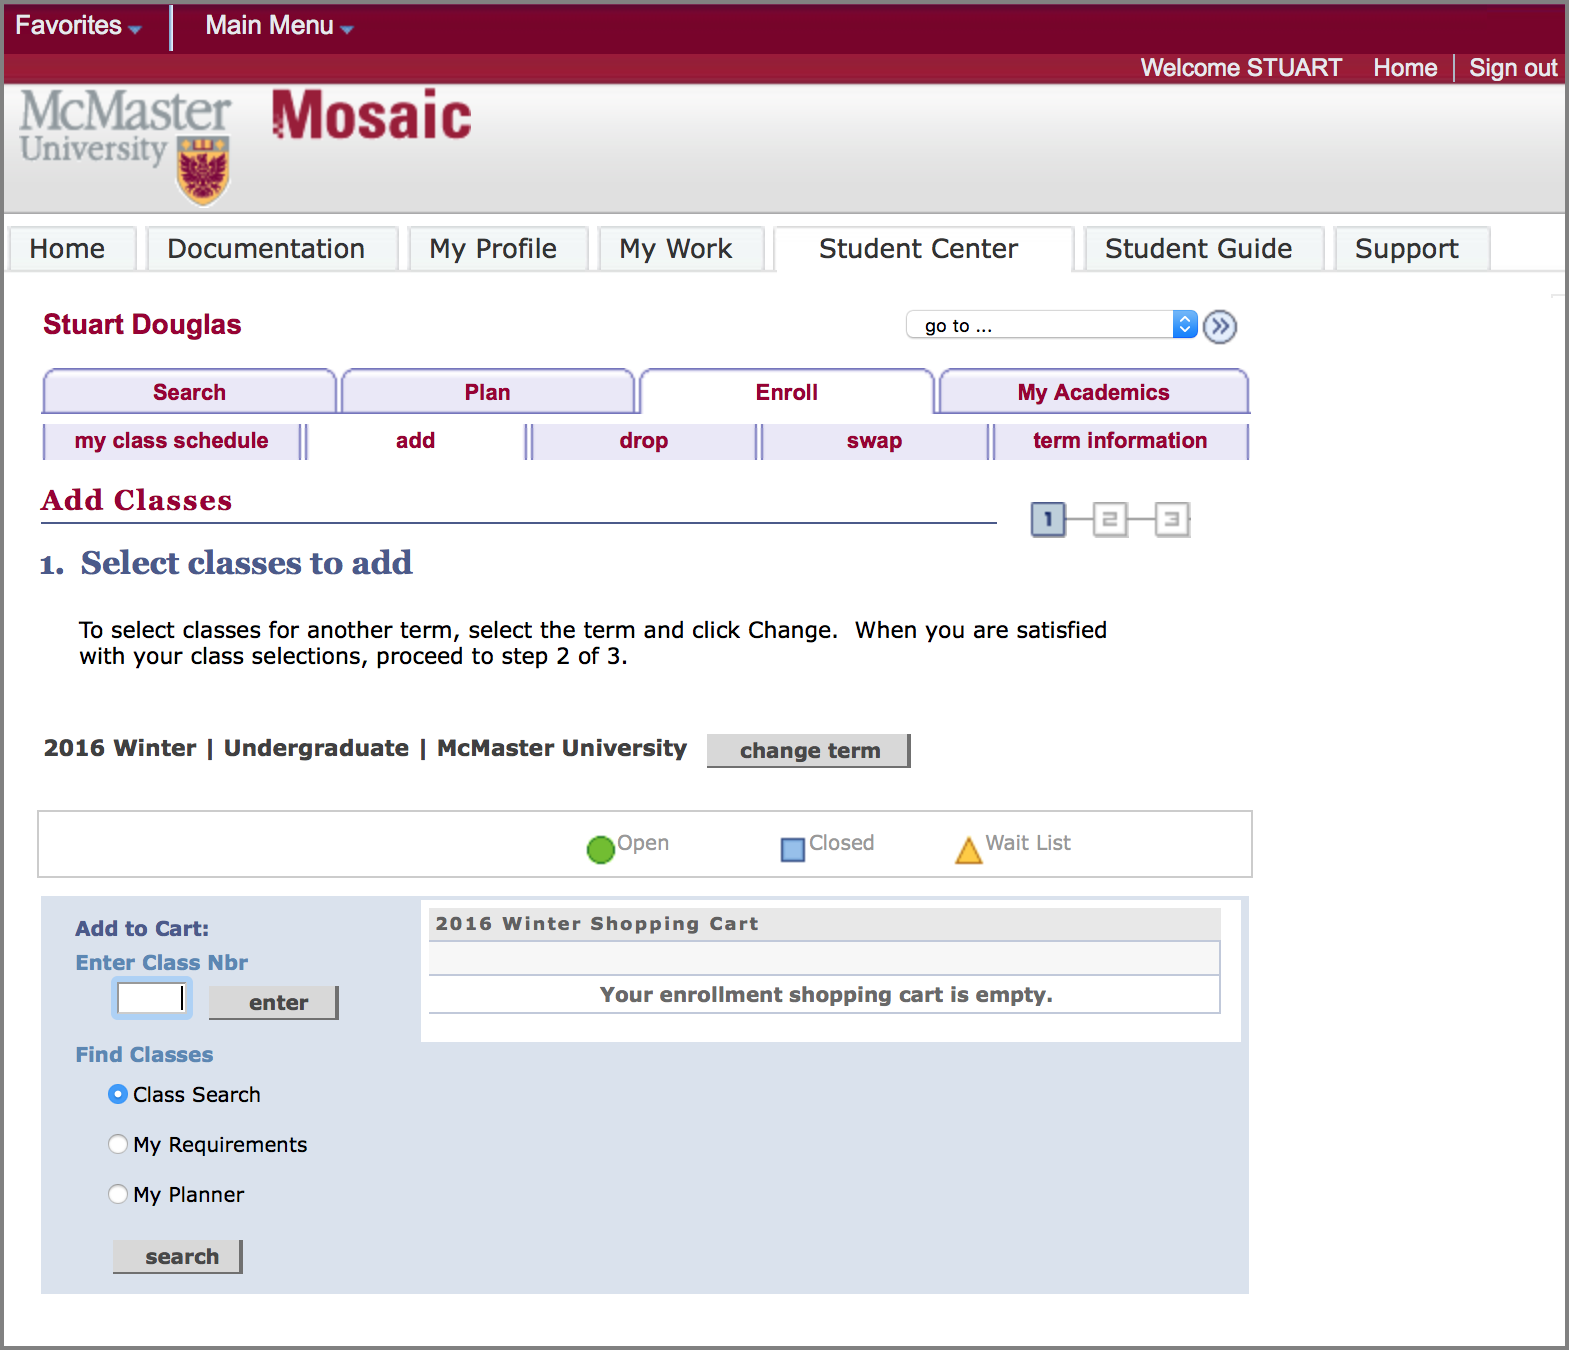
\includegraphics[width=0.9\textwidth]{MosaicScreen.png}
\end{center}
\Caption{Selecting courses to enroll in -- Mosaic}
\end{InlineColumnFigure}

\subsubsection*{Critique}
The largest usability flaws in Mosaic center around difficulty to access 
required information. Combined with an unintuitive and inconsistent navigation 
interface, the software is . The HTA for enrolling in a course demonstrates this 
through the large number of steps required to perform a routine and common task. 
Other functions are hidden behind dropdown menus, and are difficult to discover.
\\

The navigation is separated into a top navigation bar separated by user-type 
(e.g. Students and Employees). Within the student center page, functions are 
separated into modules, an effective strategy to group related functions. 
Navigating to one of the sub-functions (such as enrolling in a course) presents 
secondary and tertiary menus below the main one. Navigation within one of these 
is handled by blue text hyperlinks back to previous pages. Native back and 
forward browser functionality does not work. There is little visual indication 
of where the user is beyond the navigation bars at the top, which do not go to a 
depth sufficient to cover all pages used when performing common actions, such as 
enrolling in a course.

% =================== SubSection =================== %
\subsection*{Guelph University -- WebAdvisor}
\subsubsection*{Description}
Guelph University's course enrollment software, WebAdvisor, provides a variety 
of functions for students to manage their courses. The student page interface 
contains two columns -- a main column with course-related news, and a righthand 
column with links to each of the functions (Register for Courses, View Schedule 
etc). These ``function'' pages are one column, and may contain several sub-pages 
as processes are broken into steps. Navigating between sub-pages is done using 
native browser back and forward buttons. If an error occurs, such as no courses 
found for specific search criteria, a large box is displayed with information 
about the error and the option to search for a solution.\\

\begin{InlineColumnFigure}
\begin{center}
	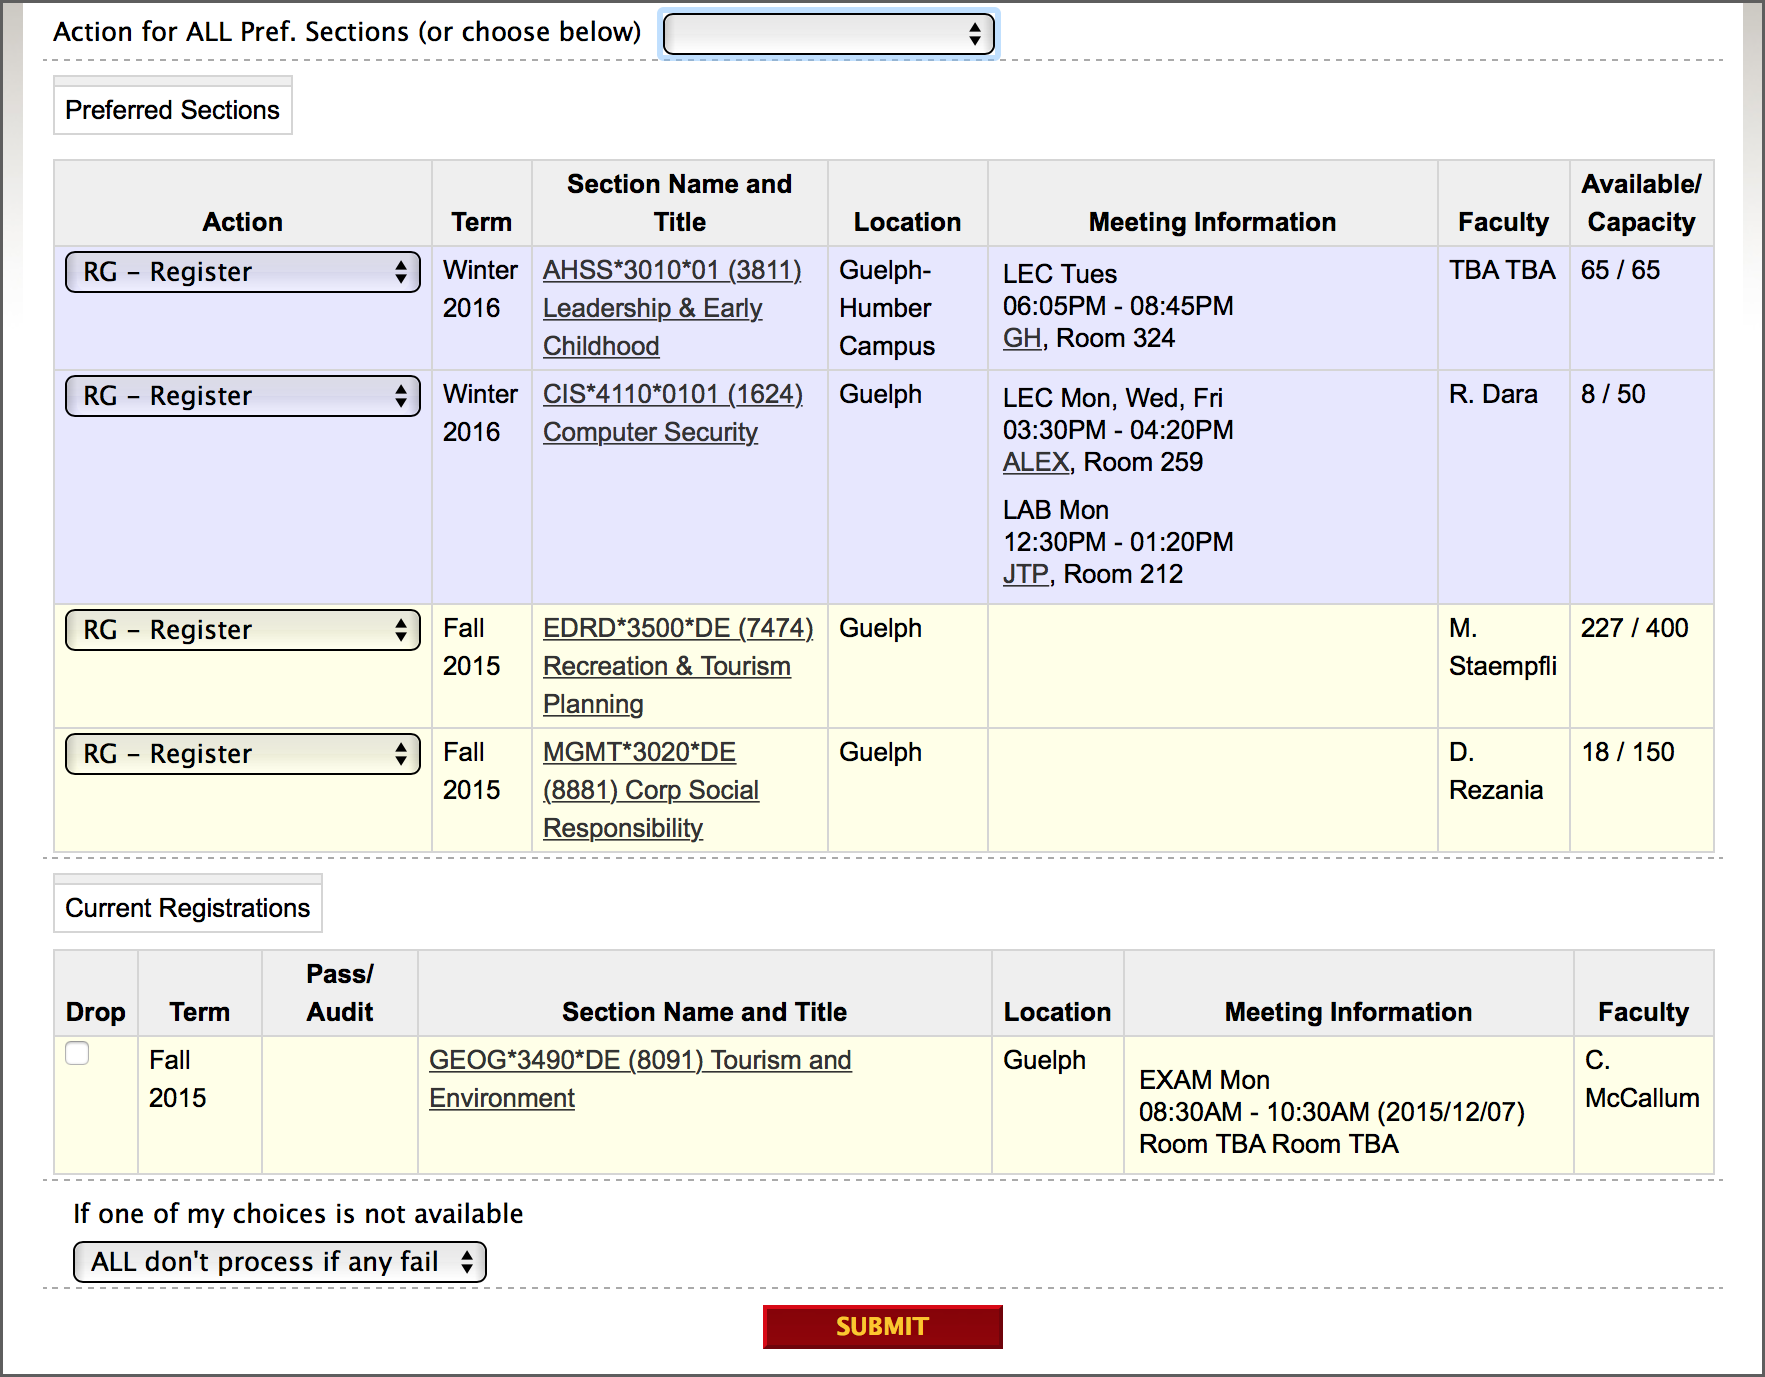
\includegraphics[width=0.9\textwidth]{WebAdvisorScreen.png}
\end{center}
\Caption{Registering for preferred courses -- WebAdvisor}
\end{InlineColumnFigure}

\subsubsection*{Critique}
There are a variety of usability issues associated with \mbox{WebAdvisor} that 
could be improved upon, especially in the area of navigation. There are also 
certain strengths to the system as compared to others surveyed. The navigation 
issues largely stem from a lack of consistent navigation elements to show the 
user where they are. For example, when enrolling in a course there are several 
steps that must be completed (refer to HTA -- WebAdvisor, Enrolling in A 
Course). The user is not aware how many steps there are total, how many they 
have completed or how many remain. Another large usability issue is an 
inefficient use of space on the main page. The visibility of important functions 
is reduced by putting all functions in a small column to the right of the main 
content. This main content contains news items, such as exam period times and 
service outages, generally information that the user is less likely to need than 
the functions beside it.\\

WebAdvisor does do some things quite well from a usability perspective however. 
One of the most common tasks is enrolling in a course, and WebAdvisor has the 
most streamlined process of all universities surveyed. Although it is not always 
clear at which step the user is at as discussed above, the process is 
straightforward and contains much fewer steps than performing a similar task 
using a different system.

% =================== SubSection =================== %
\subsection*{Carleton University -- Central}
\subsubsection*{Description}
Central is the course-management system for Carleton University. It has a 
similar feature-set to the other systems surveyed. This includes allowing users 
to enroll in courses and view their schedule. The user interface for Central 
primarily is based on text links to different pages, with very little use of 
icons or colour. The main student page is a one-column list of text links to the 
various student-related categories of functions. A tab bar at the top lets the 
user switch between different sections of the system including Student Services 
and Employee Services.\\

\begin{InlineColumnFigure}
\begin{center}
	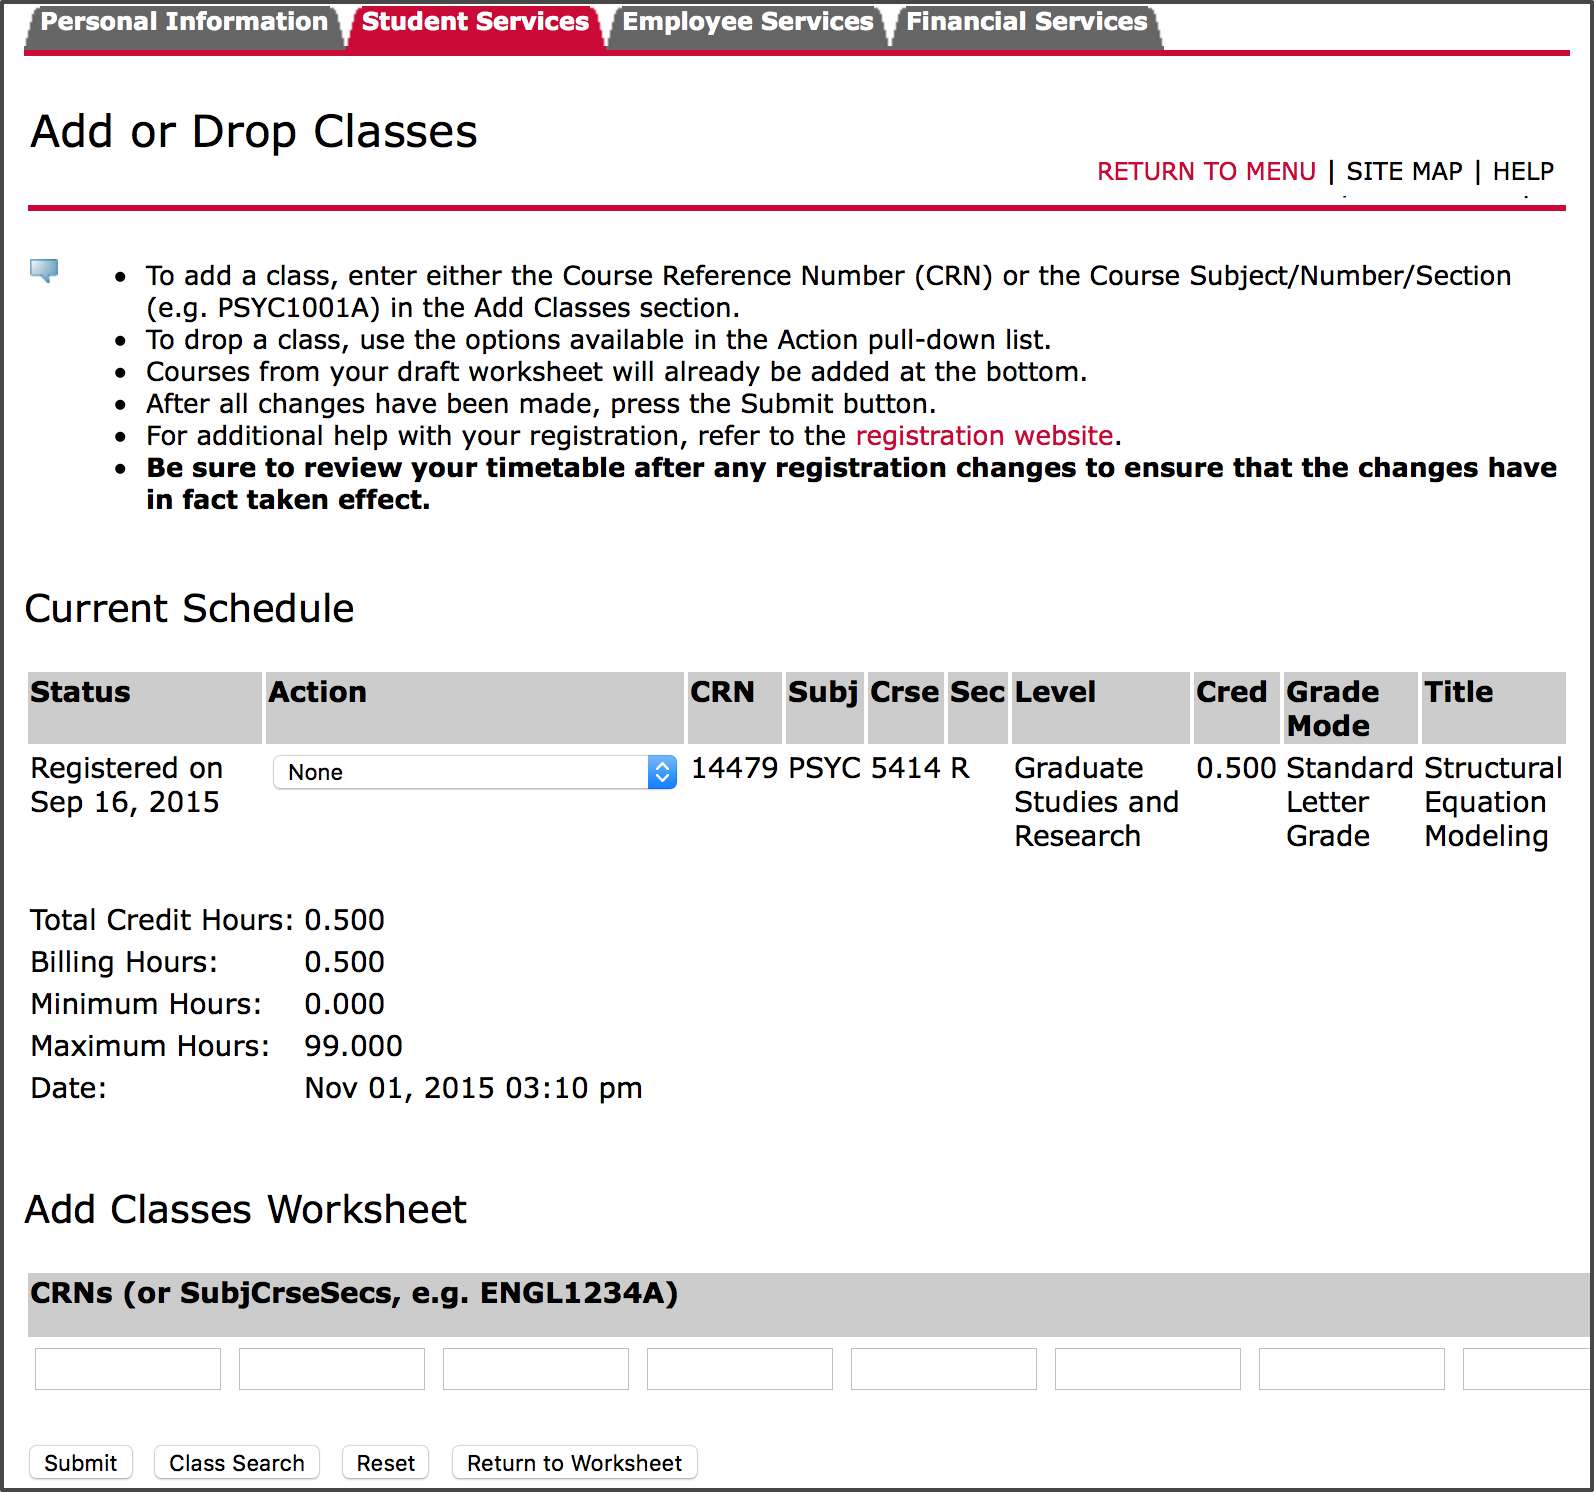
\includegraphics[width=0.9\textwidth]{CarletonScreen.png}
\end{center}
\Caption{Add courses view -- Central}
\end{InlineColumnFigure}
\vspace{2mm}

\subsubsection*{Critique}
There are a large number of prominent usability flaws in Carleton University's 
Central course-management system. Visibility of common functions on the main 
page is very low, as a long list of hyperlinks contains all the categories (e.g. 
Registration, Student Records etc) requiring the user to read each one until 
they find the correct one. Once a category is selected, then another list of 
hyperlinks to each of the functions in that category is shown (see figure 4). 
Again, the user must read through each one until they find the desired function.
\\

\begin{InlineColumnFigure}
\begin{center}
	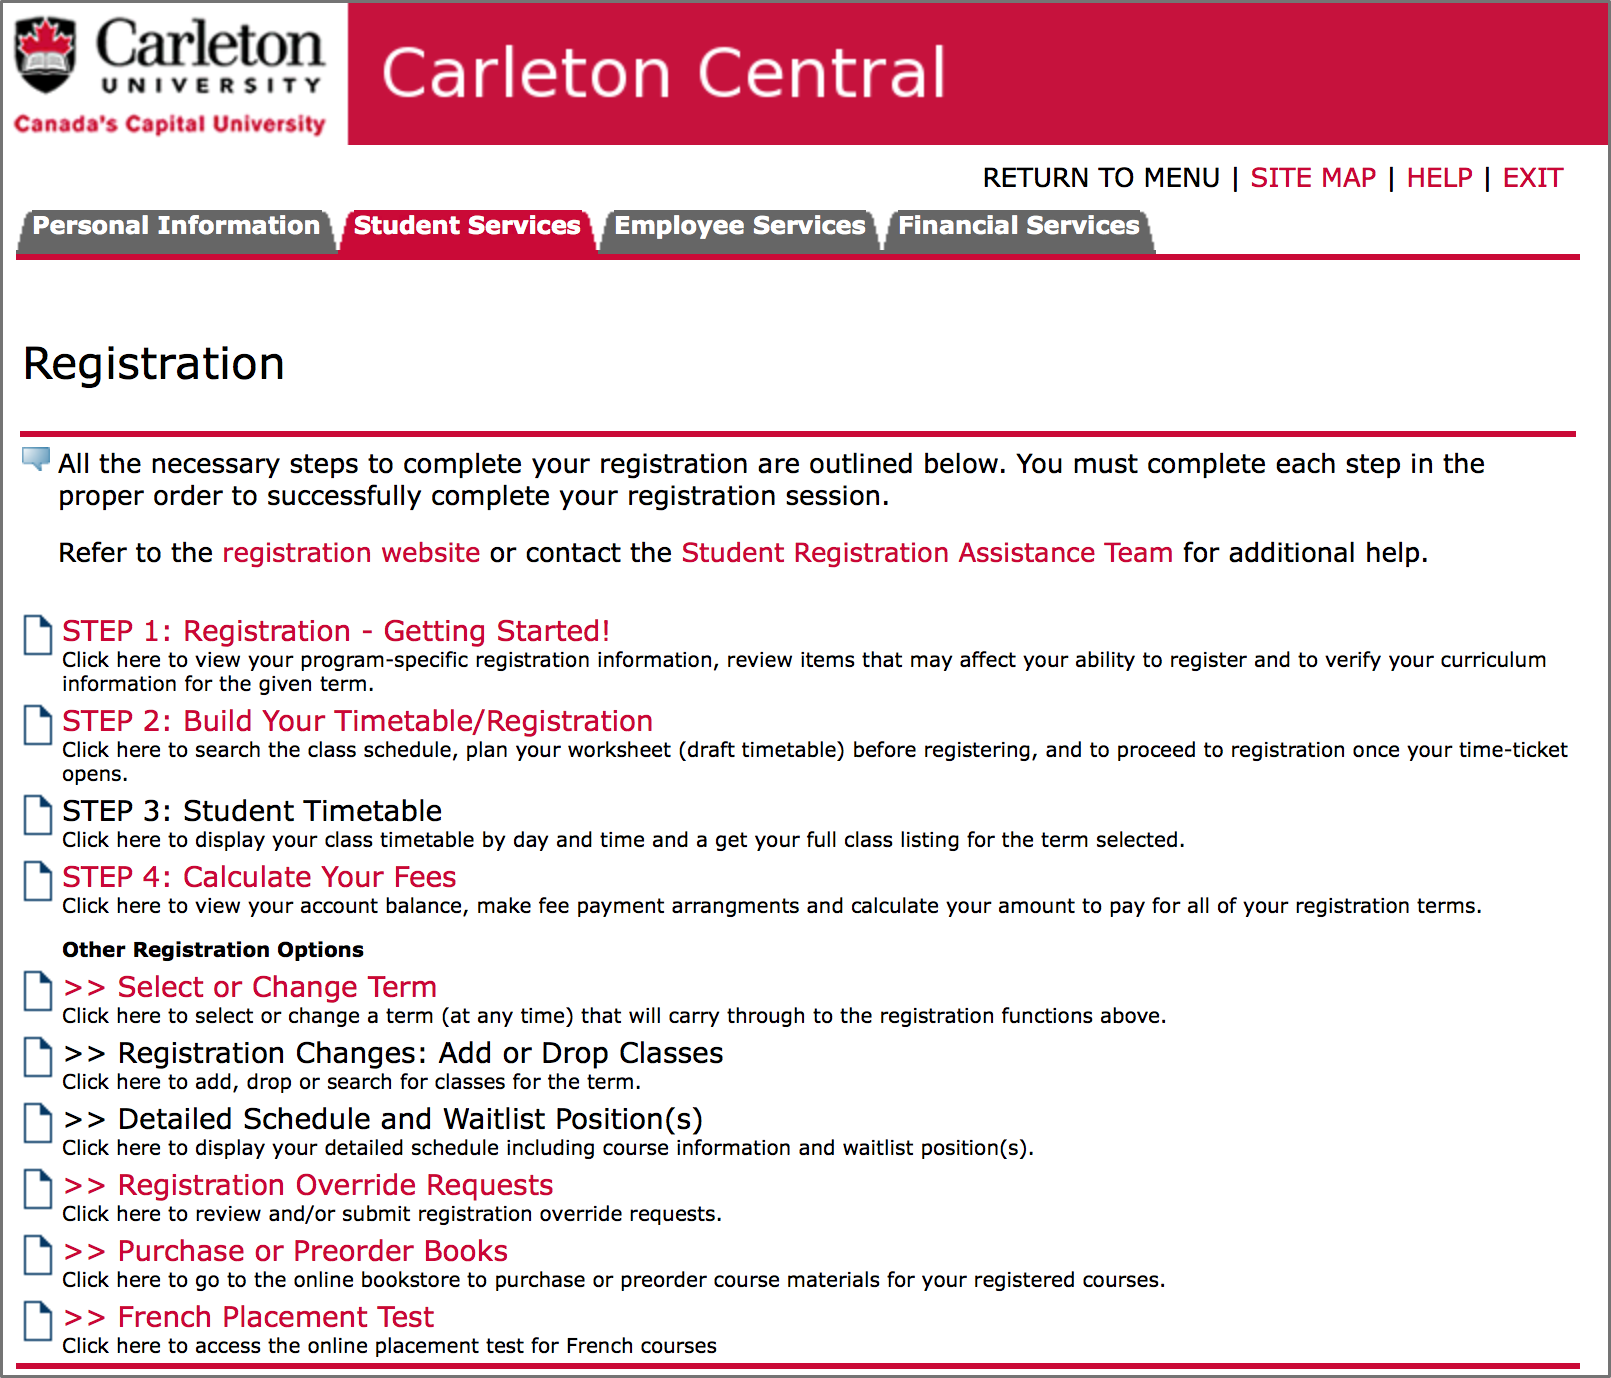
\includegraphics[width=0.9\textwidth]{CarletonScreen2.png}
\end{center}
\Caption{Registration main page -- Central}
\end{InlineColumnFigure}

Another large usability flaw is the poor mapping between many actions. For 
example, when adding a course, the user first enters a course number into one of 
several (unlabeled) input boxes, and then they click the Submit button (see 
figure 3). The submit button is aligned with other buttons for Class Search, 
which takes the user to a separate page, Reset, which undoes their changes, and 
Return to Worksheet which navigates the user to a page showing them their 
preferred courses. These buttons are not all related, and grouping them together 
may confuse the user.\\

Overall, Central is a relatively unintuitive system, requiring users to spend 
more time finding the information they need through poor mappings and a lack of 
a visual hierarchy.

% =================== SubSection =================== %
\subsection*{Waterloo University -- Quest}
\subsubsection*{Description}
The Quest system is designed to let students manage several aspects 
of their university enrollment, such as course management, financial inquiries, 
and contact information. Students can also sign up for a GO Bus pass, view their 
grades and transcript, and check the status of scholarships and other 
applications. The main page is broken up into 8 collapsible sections, 4 main 
sections (Academics, Finances, Personal Information, Admissions) with another 4 
sections in a sidebar (Holds, Finance Information, Academic Information, Other 
Useful Links). The critique will focus on enrolling in courses and viewing a 
user's course schedule. 

\begin{InlineColumnFigure}
\begin{center}
	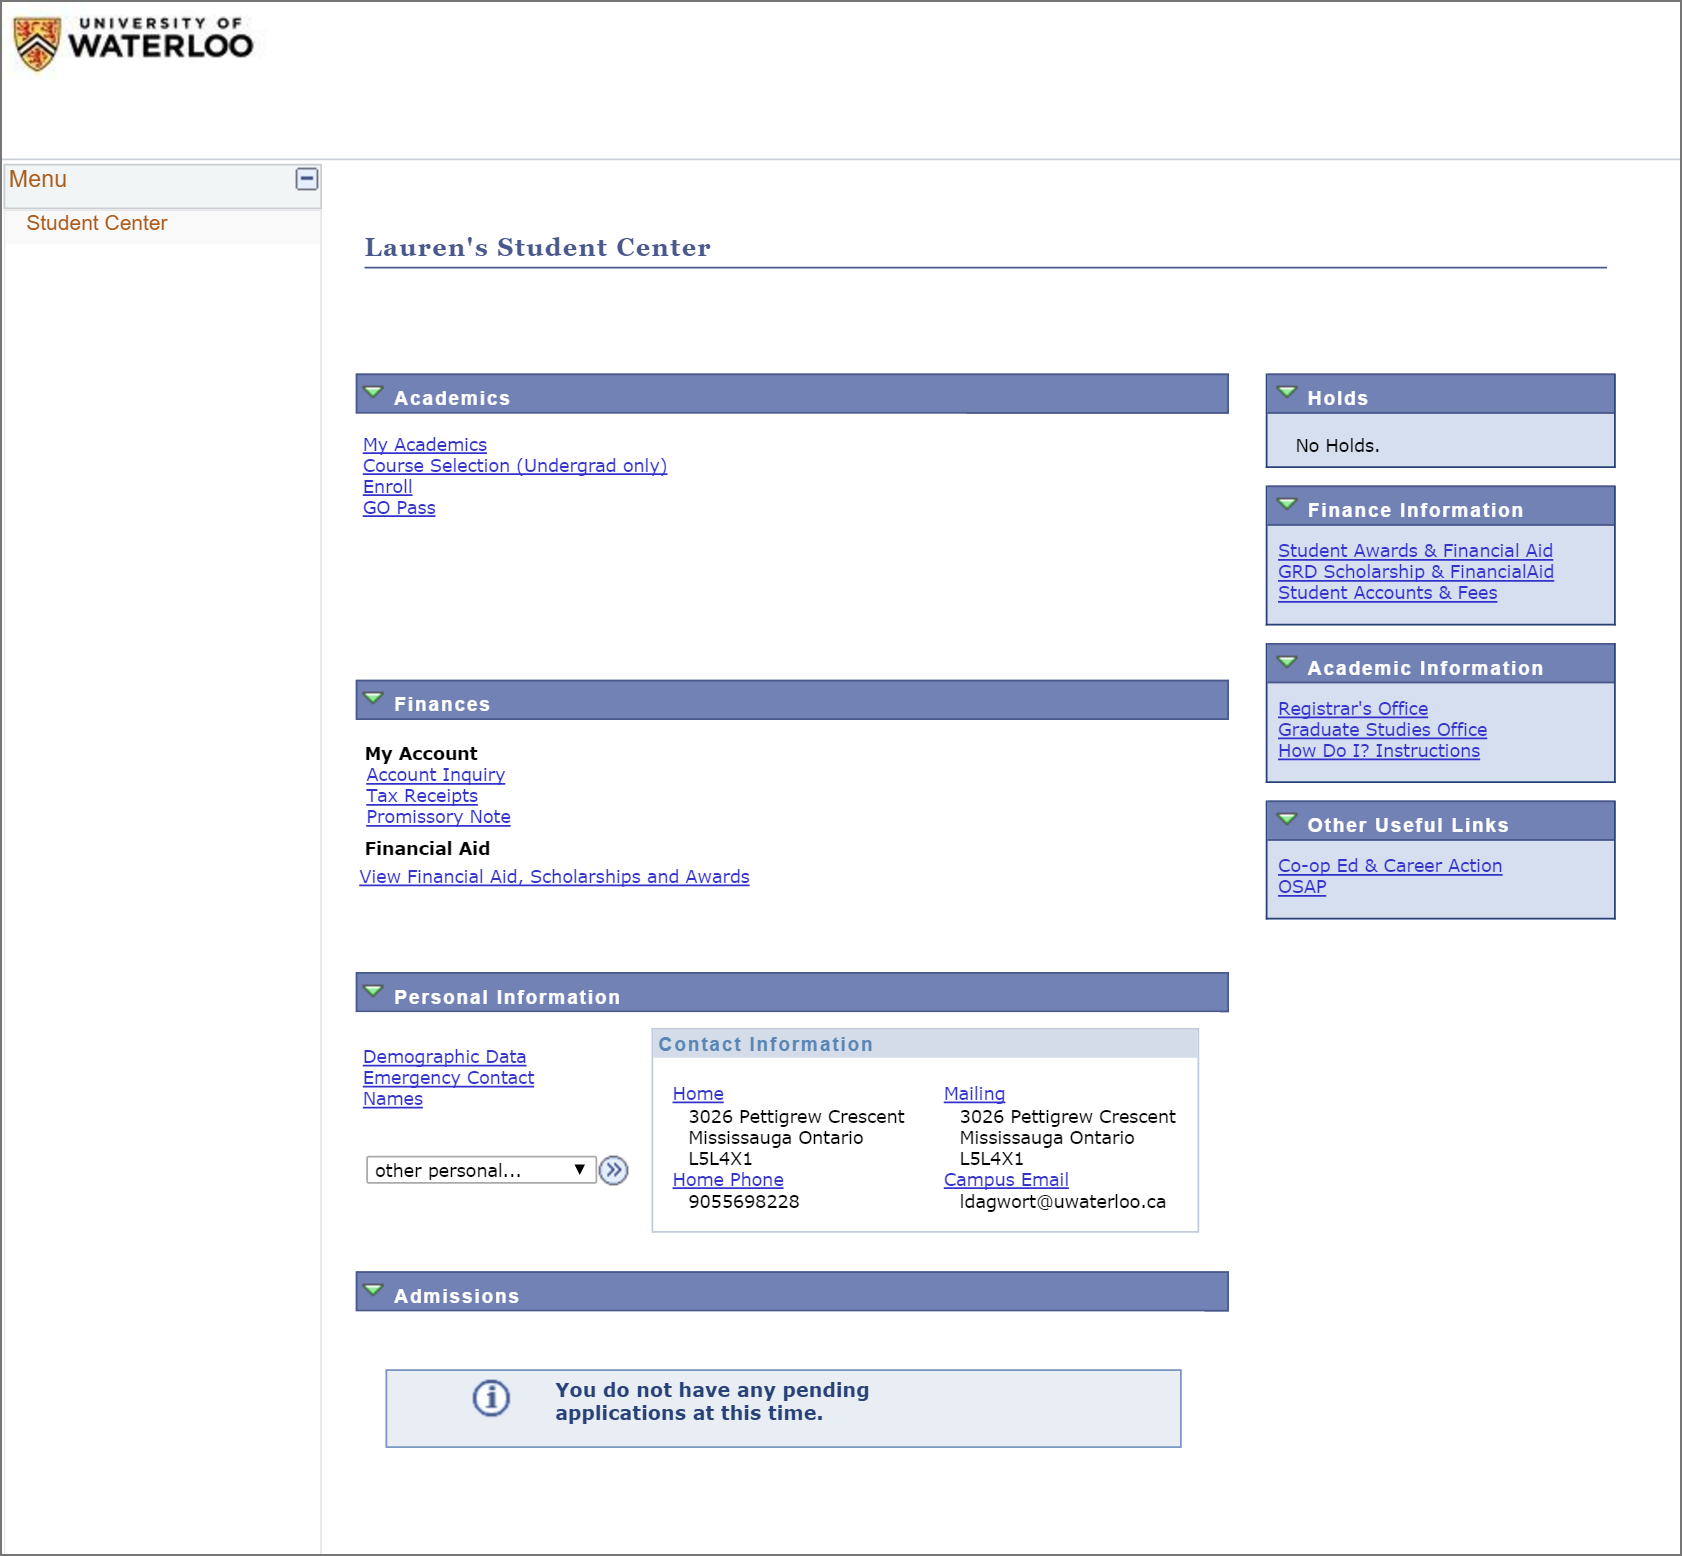
\includegraphics[width=0.9\textwidth]{WaterlooScreen.png}
\end{center}
\Caption{Student main page -- Quest}
\end{InlineColumnFigure}

\subsubsection*{Critique}
Quest has some major usability issues when it comes to providing the user to 
information and functions they can use. The system is notorious for hiding 
options and menus from the user, requiring several screens of drill down menus 
before being able to access any meaningful options. The menus look unfinished or 
poorly formatted, and it is easy to become lost and confused while navigating 
the various pages. Navigation on the main page is done using hyperlinked text, 
while traversing the deeper options is done using blue menu tabs. Native browser 
back and forward commands generally work as expected, which makes navigation a 
little more manageable. 

% =================== Section =================== 
\section*{Conclusion}
We have discussed several proposed improvements to a course-management system. 
These include a dynamic element highlighting the most-needed feature based on 
several factors, an improved layout with better indicators, and a more 
intelligent course scheduler. We have also provided a software survey for four 
Canadian university course-management systems. For each survey we critiqued the 
software as well as analyzed the two most important features via hierarchical 
task analyses, presented at the end of this paper.

\end{multicols}

\newpage

\section*{HTA - Mosaic, Enrolling in a Course}
\begin{center}
\fbox{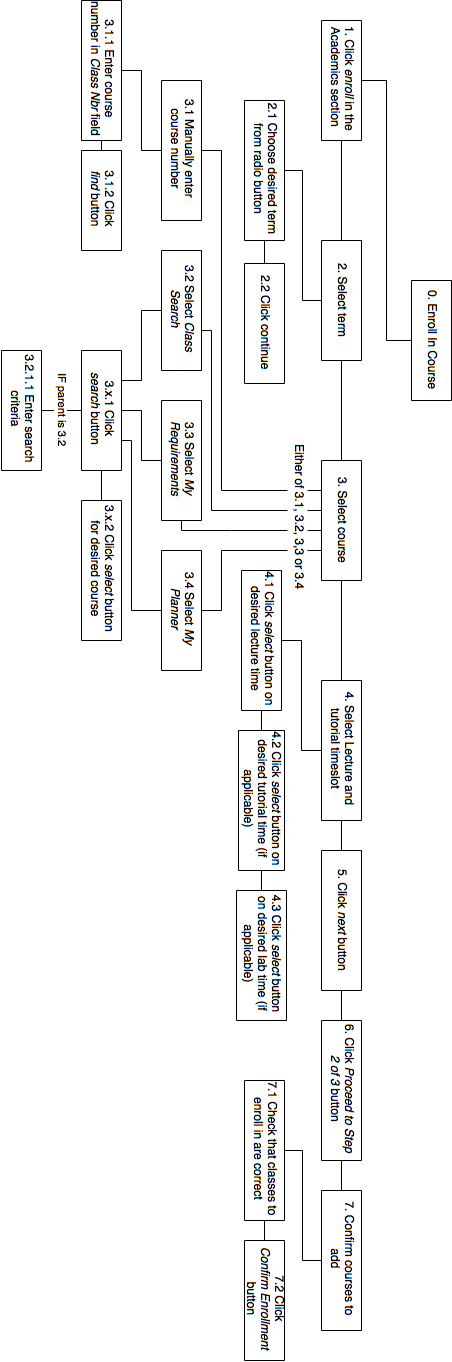
\includegraphics[height=\textheight]{MosaicEnroll.png}}
\end{center}

\section*{HTA - Mosaic, Viewing Weekly Schedule}
\begin{center}
\fbox{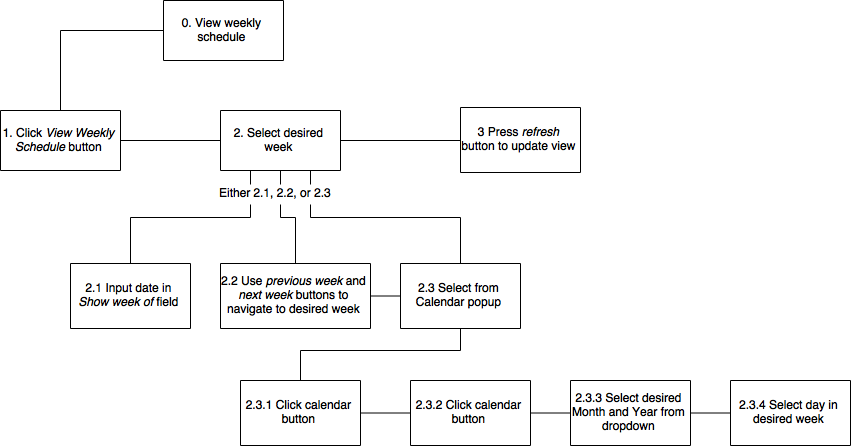
\includegraphics[width=\textwidth]{MosaicViewSchedule.png}}
\end{center}

\section*{HTA - WebAdvisor, Enrolling in a Course}
\begin{center}
\fbox{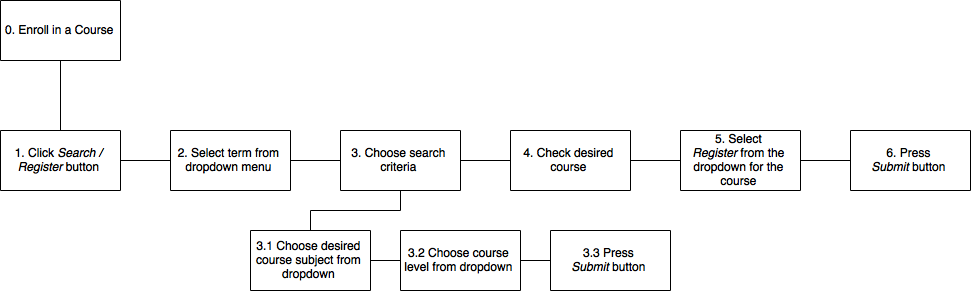
\includegraphics[width=\textwidth]{WebAdvisorEnroll.png}}
\end{center}

\section*{HTA - WebAdvisor, Viewing Weekly Schedule}
\begin{center}
\fbox{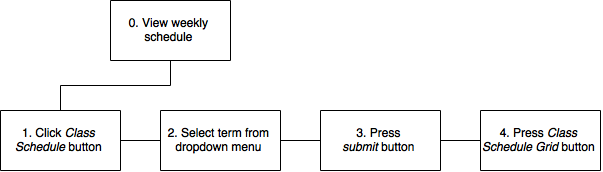
\includegraphics[width=\textwidth]{WebAdvisorViewSchedule.png}}
\end{center}

\section*{HTA - Central, Enrolling in a Course}
\begin{center}
\fbox{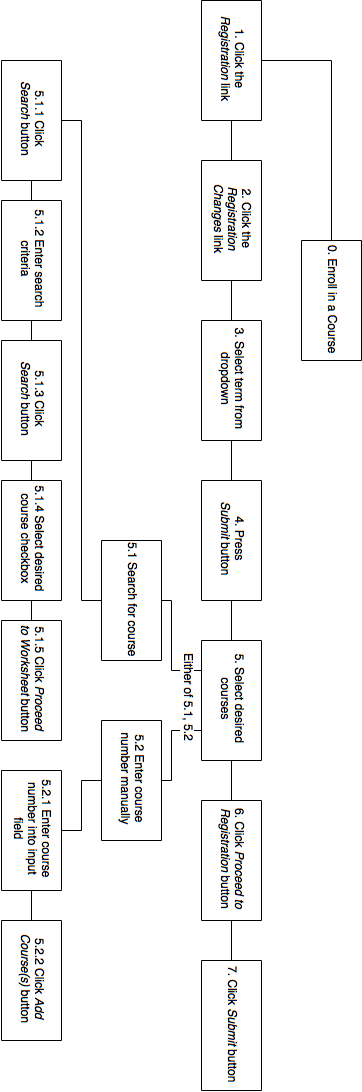
\includegraphics[height=\textheight]{CarletonEnroll.png}}
\end{center}

\section*{HTA - Central, Viewing Weekly Schedule}
\begin{center}
\fbox{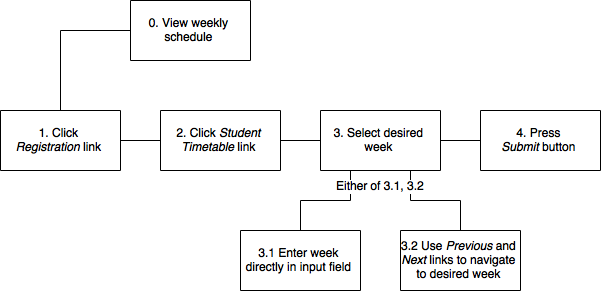
\includegraphics[width=\textwidth]{CarletonViewSchedule.png}}
\end{center}

\end{document}
